% !TEX root = ../main.tex
\chapter{Синтез лінійно-квадратичного регулятора стану}
Розглянемо математичну модель об'єкта у вигляді передаточної функції
\begin{gather*}
    W_O(s) = \frac{y(s)}{u(s)} = \frac{
    k
    }{
        (T_1 s + 1) (T_2 s + 1) (T_3 s + 1)
    } = \\ = \frac{
        k
    }{
        T_1 T_2 T_3 s^3 + \left(T_1 T_2 + T_1 T_3 + T_2 T_3\right) s^2
        + \left(T_1 + T_2 + T_3\right) s + 1
    }
\end{gather*}
Введемо нові коефіцієнти 
\begin{gather*}
    a_1 = \frac{T_1 T_2 + T_1 T_3 + T_2 T_3}{T_1 T_2 T_3} = 0.17211, 
    a_2 = \frac{T_1 + T_2 + T_3}{T_1 T_2 T_3} = 0.00889 \\
    a_3 = \frac{1}{T_1 T_2 T_3} = 0.00014, 
    b = \frac{k}{T_1 T_2 T_3} = 0.00127
\end{gather*}
після чого цю передаточну функцію можна записати наступним чином:
\begin{gather*}
    W_O(s) = \frac{b}{s^3 + a_1 s^2 + a_2 s + a_3} = \frac{y(s)}{u(s)}
\end{gather*}
Введемо нову змінну $X(s) = \frac{u(s)}{s^3 + a_1 s^2 + a_2 s + a_3} = \frac{y(s)}{b}$, звідки
\begin{gather*}
    u(s) = \left(s^3 + a_1 s^2 + a_2 s + a_3\right) X(s)
\end{gather*}
Виконавши зворотнє перетворення Лапласа, отримаємо
\begin{gather*}
    \frac{d^3 x(t)}{dt^3} = u(t) - a_1 \frac{d^2 x(t)}{dt^2} - a_2 \frac{d x(t)}{dt} - a_3 x(t)
\end{gather*}
Введемо фазові змінні $x_1(t) = x(t)$, $x_2(t) = \frac{d x(t)}{dt}$, $x_3(t) = \frac{d^2 x(t)}{dt^2}$,
причому $\frac{d x_1(t)}{dt} = x_2(t)$, $\frac{d x_2(t)}{dt} = x_3(t)$,
$\frac{d x_3(t)}{dt} = -a_3 x_1(t) - a_2 x_2(t) - a_1 x_3(t) + u(t)$. Запишемо ці рівності у векторно-матричній формі:
\begin{gather}\label{eq:state_space}
    \begin{bmatrix}
        \frac{d x_1(t)}{dt} \\ \frac{d x_2(t)}{dt} \\ \frac{d x_3(t)}{dt}
    \end{bmatrix} = 
    \begin{bmatrix}
        0 & 1 & 0 \\
        0 & 0 & 1 \\
        -a_3 & -a_2 & -a_1
    \end{bmatrix}
    \begin{bmatrix}
        x_1 \\ x_2 \\ x_3
    \end{bmatrix} + 
    \begin{bmatrix}
        0 \\ 0 \\ 1
    \end{bmatrix} u(t)
    \Leftrightarrow
    \frac{d \vec{x}(t)}{dt} = A \vec{x}(t) + \vec{b} u(t)
\end{gather}
Виконаємо дискретизацію рівняння \eqref{eq:state_space}, використавши період квантування,
який було визначено в резонансному методі ($T_0 = 11.13496$):
\begin{gather}
    \vec{x}\left(\left[k+1\right]T_0\right) = F \vec{x}\left(kT_0\right) + \vec{g} u\left(k T_0\right)
\end{gather}
де $F = e^{A T_0}$, $\vec{g} = \int_0^{T_0} e^{A t} \vec{b} dt = A^{-1} \left(e^{A T_0} - I\right) \vec{b}$.
Обчислимо значення $F$ та $\vec{g}$:
\begin{gather*}
    F = \begin{pmatrix}
        0.98025  & 9.79083  & 33.05948 \\
        -0.00452 & 0.68649  & 4.1009 \\
        -0.00056 & -0.04096 & -0.01933
    \end{pmatrix}, \;
    \vec{g} = \begin{pmatrix}
        144.46778 \\ 33.05948 \\ 4.1009
    \end{pmatrix}
\end{gather*}

Синтез лінійно-квадратичного регулятора стану 
\begin{gather}\label{eq:lin_quad_reg}
    u\left(k T_0\right) = -\vec{K}_p \vec{x}\left(k T_0\right) = 
    - \begin{bmatrix}
        K_1 & K_2 & K_3
    \end{bmatrix}
    \begin{bmatrix}
        x_1\left(k T_0\right) \\
        x_2\left(k T_0\right) \\
        x_3\left(k T_0\right)
    \end{bmatrix}
\end{gather}
виконаємо за рекурентною процедурою
\begin{gather*}
    \vec{K}_p (k) = \left(q_3 + \vec{g}^T L\left([k+1]T_0\right) \vec{g}\right)^{-1}
    \vec{g}^T L\left((k+1)T_0\right) F \\
    L\left(k T_0\right) = F^T L\left([k+1]T_0\right) F + Q_2 - 
    F^T L\left([k+1]T_0\right) \vec{g} \cdot \vec{K}_p (k)
\end{gather*}
при початковому значенні матриці $L\left(n T_0\right) = Q_1$, де вагові матриці
$Q_1$, $Q_2$ та коефіцієнт $q_3$ обираються для забезпечення швидкості мінімізації квадратичного критерію оптимальності
\begin{gather*}
    I = \vec{x}^T \left(nT_0\right) Q_1 \vec{x} \left(nT_0\right) + 
    \sum_{k=0}^{n-1} \left(
        \vec{x}^T \left(k T_0\right) Q_2 \vec{x} \left(k T_0\right) + q_3 u^2 \left(k T_0\right)
    \right)
\end{gather*}

За наведеною рекурентною процедурою отримаємо 
\begin{gather*}
    \vec{K}_p = \begin{bmatrix}
        0.00278 & 0.03643 & 0.15089
    \end{bmatrix}
\end{gather*}
На основі рівнянь \eqref{eq:state_space} та \eqref{eq:lin_quad_reg}
маємо рівняння стану замкненої системи:
\begin{gather*}
    \vec{x}\left([k+1]T_0\right) = \left(F - \vec{g} \cdot \vec{K}_p \right) \vec{x}\left(kT_0\right)
\end{gather*}
Користуючись цим рівнянням, змоделюємо поведінку системи при різних ненульових початкових умовах:
\begin{center}
    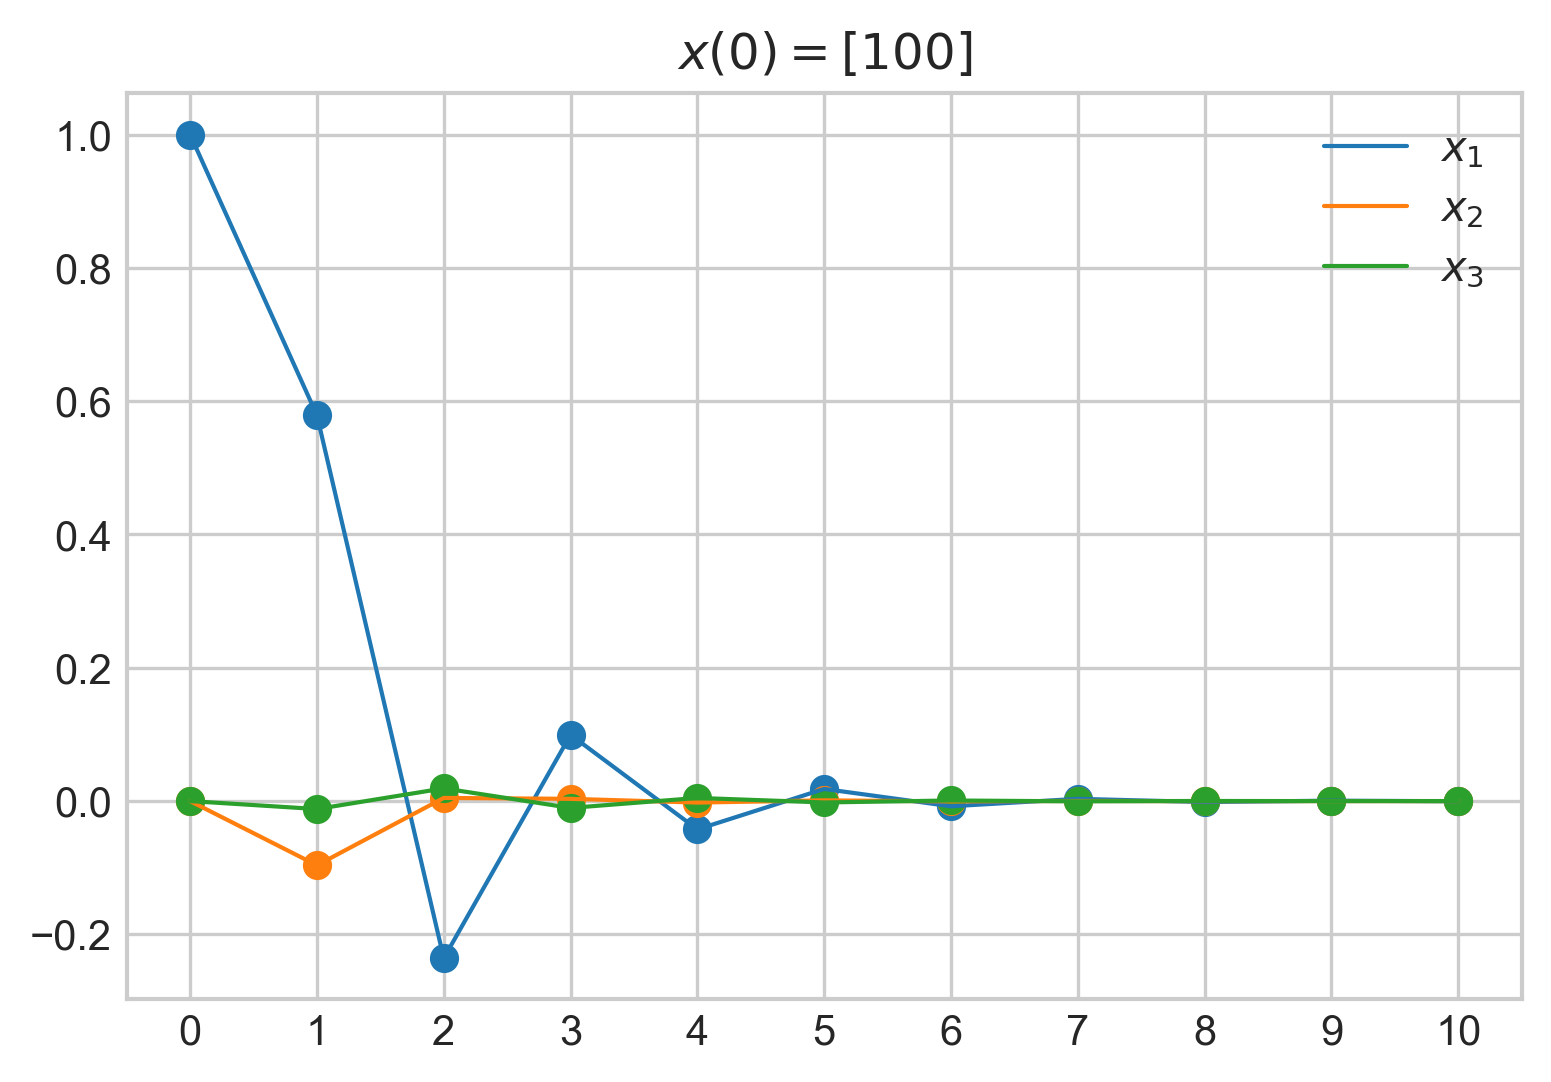
\includegraphics[scale=0.9]{pics/lin_quad_model_[1 0 0].png} \\
    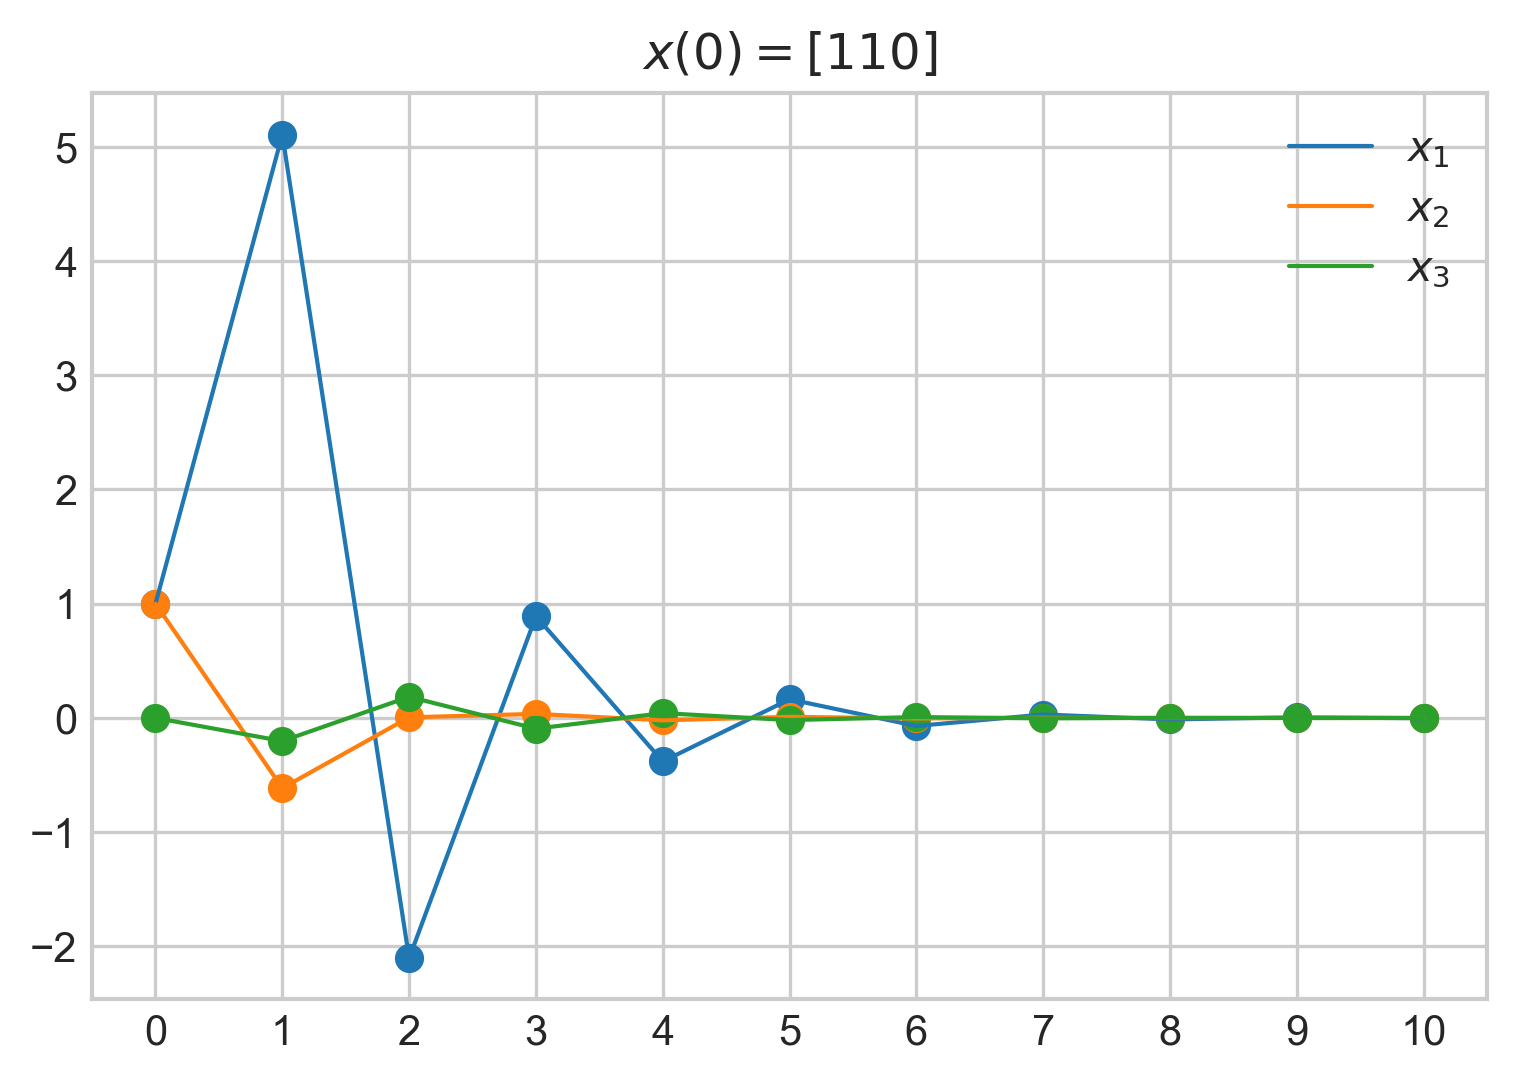
\includegraphics[scale=0.9]{pics/lin_quad_model_[1 1 0].png} \\
    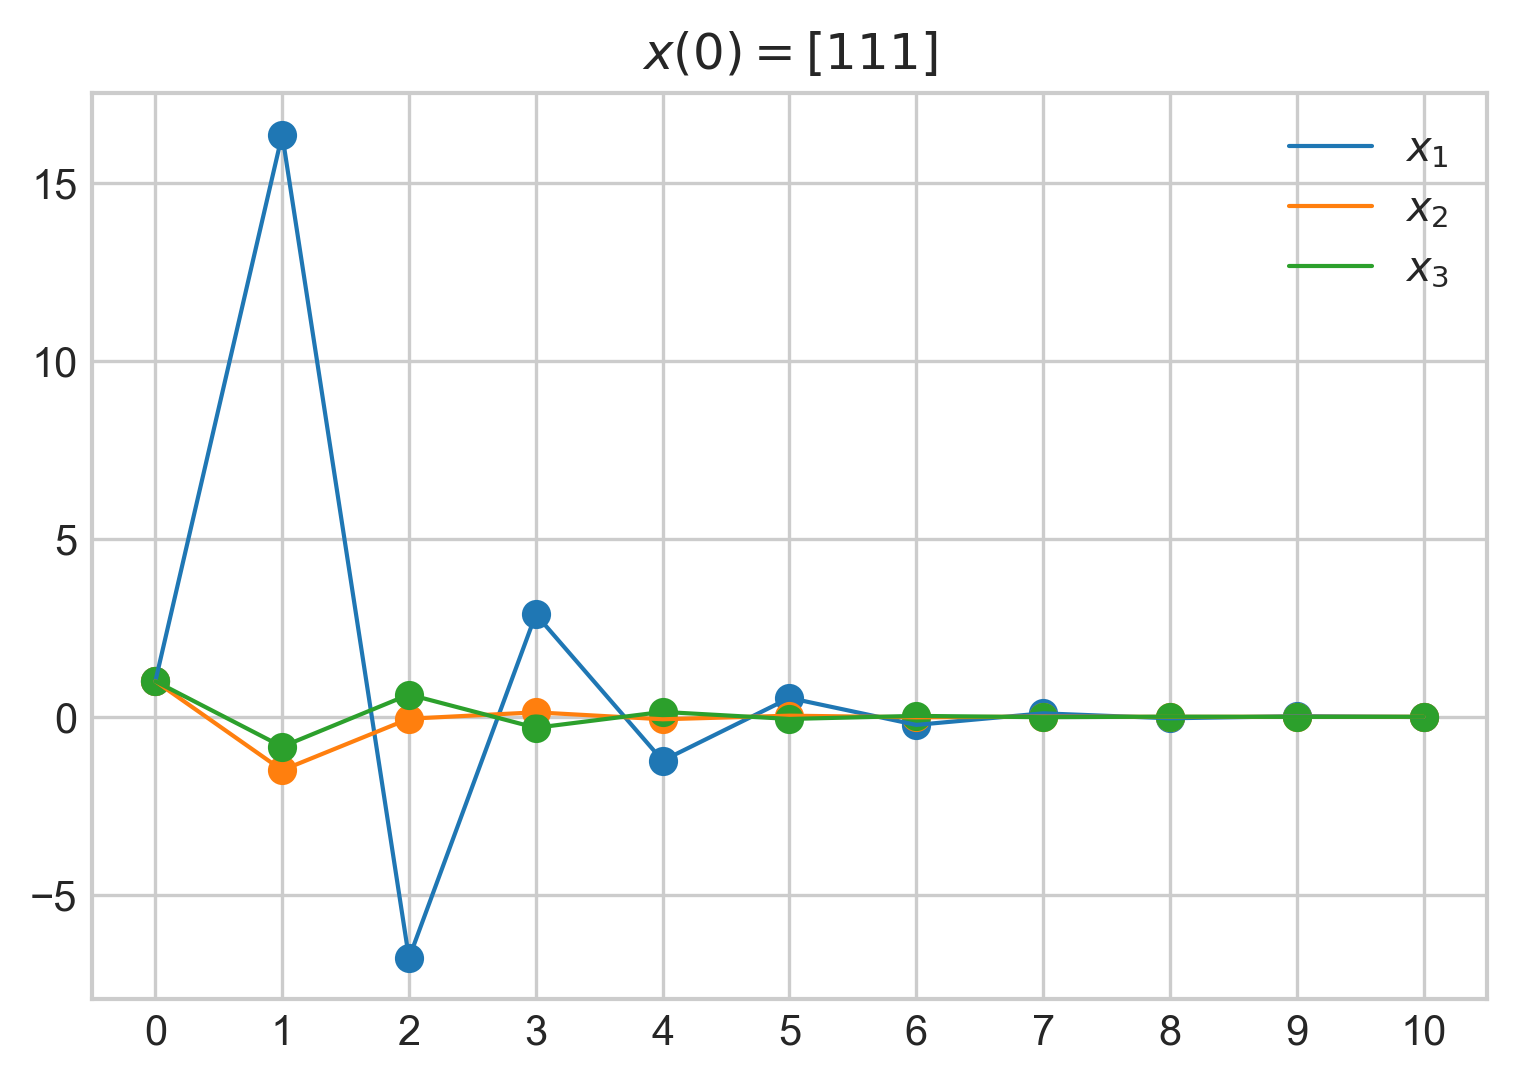
\includegraphics[scale=0.9]{pics/lin_quad_model_[1 1 1].png}
\end{center}